\documentclass[./../../paper.tex]{subfiles}
\graphicspath{{\subfix{./../../figures/}}}

\begin{document}
Having discussed the previous work on generating counterfactual sequences, a couple of challenges emerge. First, we need to generate on a set of criteria and therefore, require complex loss and evaluation metrics, that may or may not be differiantiable. Second, they cannot to be logically impossible, given the data set. Hence, we have to restrict the space to counterfactuals to viable solutions, while being flexible enough to not just be copies of already existing data instances. Third, using domain knowledge of the process significantly reduces the practicality of any solution. Therefore, we have to develop an approach, which requires only the given log as input while not relying on process specific domain knowledge. This begs the question, whether there is a process-agnostic method to generate sequential counterfactuals that are viable. In terms of specific research questions we try to answer:

\begin{itemize}
    \item[RQ:] Which existing counterfactual approaches can be applied to generate sequences?
    \begin{itemize}
        \item[RQ1:] Which evaluation metric, reflects the viability of counterfactuals?
        \item[RQ2:] To which extend do viable counterfactuals align with domain experts?  
    \end{itemize}
\end{itemize}

\noindent We approach these questions, by proposing a schematic framework which allows the exploration of several independent components. \autoref{fig:framework_simplified} shows the conceptual framework of the base approach visually.

\begin{figure}[htb]
    \label{fig:framework_simplified}
    \centering
    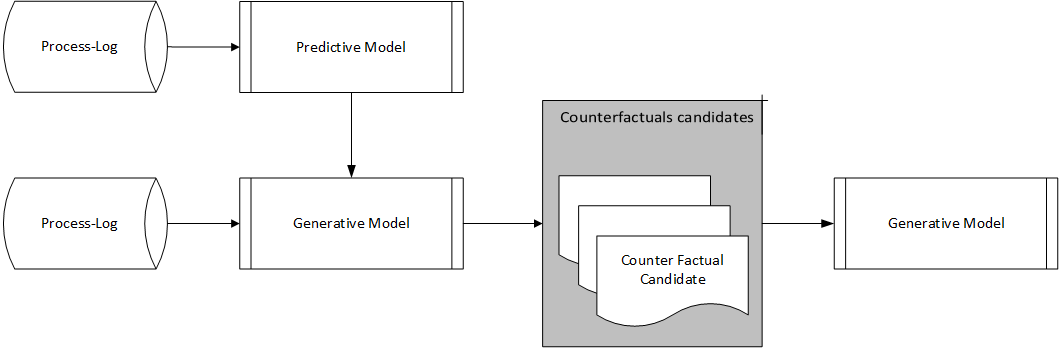
\includegraphics[width=0.9\textwidth]{figures/framework_simplified.png}
    \caption{This figure shows a simplified schematic representation of the framework which is explored in this thesis.}
\end{figure}

\noindent The framework contains three parts. First, we need a pretrained predictive component which we aspire to explain. The component should be capable of \emph{accurately} predicting the outcome of a process at any step. The accuracy-condition is favorable but not necessary. If the component is accurately modelling the real world, we can draw real-world conclusions from the explanations generated. If the component is inaccurate, the counterfactuals only explain the prediction decisions and not the real world. The second part requires a generative component. The generative component needs to generate viable sequential counterfactuals which are logically \emph{plausible}. A plausible counterfactual is one whose outcome can be  predicted by the predictive component. If the predictive component cannot predict the counterfactual sequence, we can assume that the generative model is \emph{unfaithful} to the predictive component, we want to explain. The third component is the evaluation metric upon which we decide the viability of the counterfactual candidates.

\end{document}